\documentclass[border=5px]{standalone}
\usepackage{tikz}
\usetikzlibrary{arrows,arrows.meta,automata,positioning}
\begin{document}
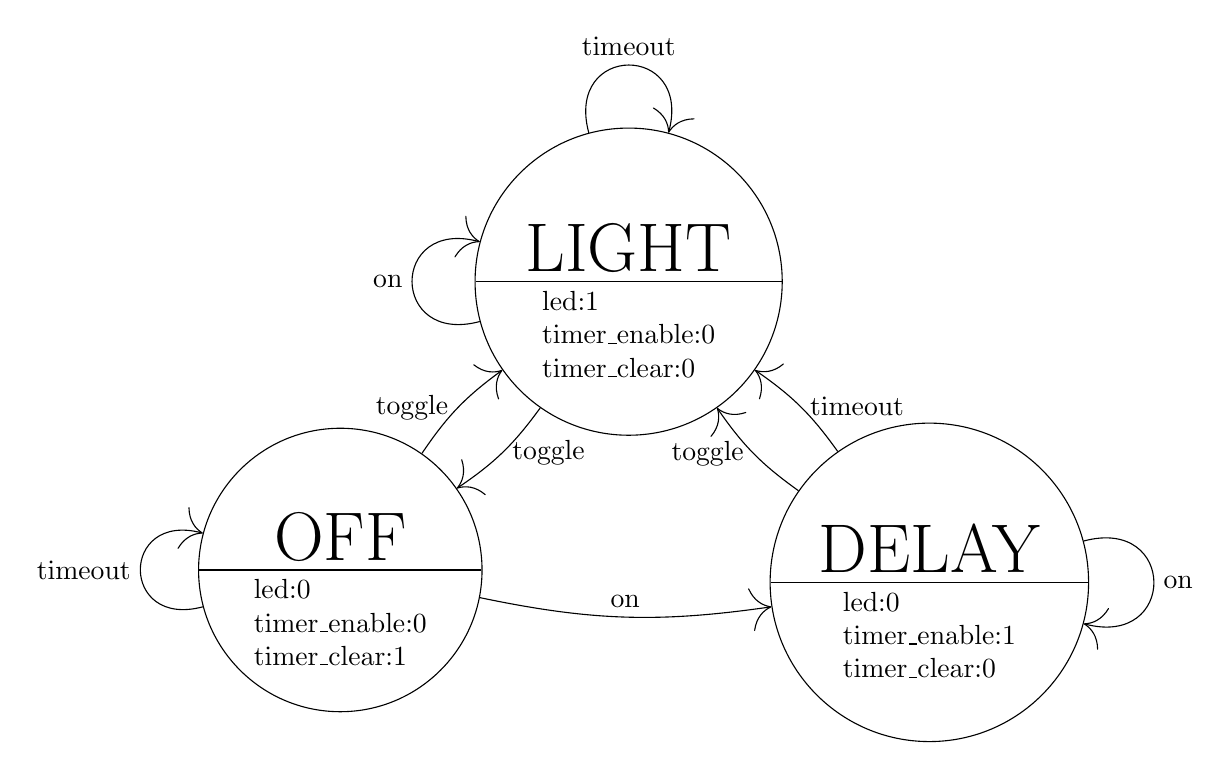
\begin{tikzpicture}
\tikzstyle{every circle split node}=[minimum size=3cm, draw, align=left] 
\tikzstyle{every path}=[arrows={->[scale=3]}, bend angle=10] 
\tikzset{every loop/.style={min distance=5mm, looseness=3}}
\node [circle split] (OFF) {\Huge OFF \nodepart{lower} led:0\\timer\_enable:0\\timer\_clear:1};
\node [circle split, above right=of OFF] (LIGHT) {\Huge LIGHT \nodepart{lower} led:1\\timer\_enable:0\\timer\_clear:0};
\node [circle split, below right=of LIGHT] (DELAY) {\Huge DELAY \nodepart{lower} led:0\\timer\_enable:1\\timer\_clear:0};
\path (OFF) edge [bend left] node [left] {toggle} (LIGHT);
\path (LIGHT) edge [bend left] node [right] {toggle} (OFF);
\path (DELAY) edge [bend left] node [left] {toggle} (LIGHT);
\path (OFF) edge [bend right] node [above] {on} (DELAY);
\path (DELAY) edge [bend right] node [right] {timeout} (LIGHT);
\path (OFF) edge [loop left] node [left] {timeout} (OFF);
\path (LIGHT) edge [loop left] node [left] {on} (LIGHT);
\path (LIGHT) edge [loop above] node [above] {timeout} (LIGHT);
\path (DELAY) edge [loop right] node [right] {on} (DELAY);
\end{tikzpicture}
\end{document}
